\documentclass[a4paper,12pt]{article}
\usepackage{graphicx}
\usepackage{fancyhdr}
\usepackage{xcolor}
\usepackage[table]{xcolor}
\usepackage{hyperref}
\usepackage{indentfirst}

\pagestyle{fancy}

\fancyhf{} 
\fancyfoot[L]{\textcolor{teal}{\rule[0mm]{0.45\linewidth}{2pt}}} 
\fancyfoot[R]{\textcolor{teal}{\rule[0mm]{0.45\linewidth}{2pt}}} 

\fancyfoot[C]{\thepage}

\renewcommand{\contentsname}{\textcolor{teal}{Table of Contents}}

\begin{document}

\begin{titlepage}
    \begin{center}
        \vspace*{2cm}

        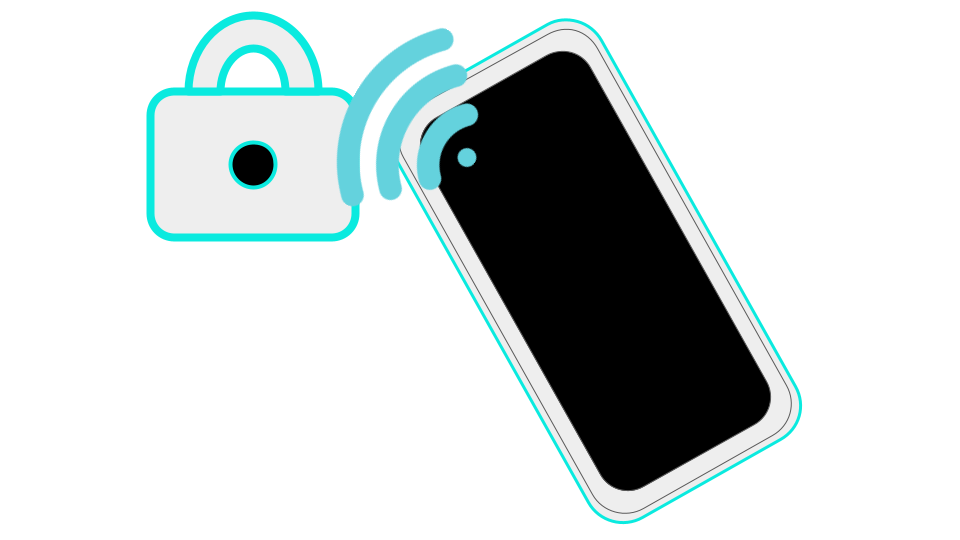
\includegraphics[width=0.8\textwidth]{./img/slimg.png}\\[1cm]

        {\Huge \textbf{Smart Lock}}\\[0.5cm]
        {\textcolor{teal}{\Large A Cloud-Based Key}}\\[1.5cm]

        {\LARGE \textbf{Group 5}}\\[0.5cm]
        {\Large \textit{Nathaniel Laurente, Adam Wu, Neena Nguyen, Jackson Kennedy}}\\[2cm]

        {\Large \today}
    \end{center}
\end{titlepage}

\newpage
\pagenumbering{arabic}
\pagestyle{fancy}      



% BEGIN DOCUMENT -------------------------------------------------------------------------


\section{Front Matter}

% Executive Summary
\section*{\textcolor{gray}{Executive Summary}}

In an era where security and convenience are necessary, traditional lock-and-key systems are becoming outdated. Lost keys, forgotten access codes, and lack of remote control present serious challenges for homeowners and businesses alike. Our Auto Smart Lock project is a solution designed to enhance security while offering friendly user accessibility.
\newline
Our goal is to develop a smart lock that integrates modern authentication methods with remote access capabilities. By leveraging an ESP32-C3 microcontroller in conjunction with Firebase cloud services, our smart lock enables users to lock and unlock their doors from anywhere, eliminating the risks associated with traditional keys.
\newline

At the core of our smart lock is an ESP32-C3 microcontroller, which connects to WiFi and Firebase cloud services to securely manage lock and unlock commands. When a user enters a PIN or sends a command from their phone, the system checks if the code is valid. If it is, the solenoid lock is triggered, unlocking the door. We’ve designed the lock to be fast, secure, and easy to install, with a 3D-printed casing to house the components.
\newline

Before finalizing the prototype, we are running key tests to ensure everything works smoothly. These tests check if the phone properly connects to the lock, if the lock responds quickly, if multiple users can access it without conflicts, and if temporary PINs expire when they should. Our next steps include assembling all parts, optimizing performance, and making sure the system is fully secure and reliable. By the end of Winter 2025, we aim to have a fully functional smart lock prototype that provides a safer, smarter, and more convenient way to secure homes.

% Ethics Statement
\newpage
\section*{\textcolor{gray}{Ethics Statement for Smart Lock Project}}
Our Smart Lock is designed to enhance security and convenience for users while upholding ethical standards in privacy, safety, and accessibility. We recognize our responsibility to develop and deploy technology that prioritizes ethical considerations in the following ways:

\textcolor{teal}{\subsection*{Privacy and Data Protection}}
We are committed to safeguarding user privacy by:
\begin{itemize}
    \item Minimizing data collection to only essential information required for functionality.
    \item Implementing encryption and secure authentication methods to prevent unauthorized access.
    \item Ensuring that user data is never shared or sold to third parties without explicit consent.
\end{itemize}

\textcolor{teal}{\subsection*{Security and Reliability}}
To maintain the integrity of the smart lock system, we will:
\begin{itemize}
    \item Use cybersecurity measures to prevent hacking and tampering.
    \item Regularly update software and firmware to address potential vulnerabilities.
    \item Ensure the lock functions reliably under various conditions to prevent accidental lockouts or failures.
\end{itemize}

\textcolor{teal}{\subsection*{User Safety and Accessibility}}
We aim to create a system that is safe and inclusive by:
\begin{itemize}
    \item Designing intuitive user interfaces for easy access by individuals with different levels of technical proficiency.
    \item Ensuring compliance with accessibility standards for individuals with disabilities.
\end{itemize}

\textcolor{teal}{\subsection*{Ethical Use and Non-Discrimination}}
The smart lock must be used ethically and responsibly by:
\begin{itemize}
    \item Preventing misuse that could lead to unauthorized surveillance or discrimination.
    \item Avoiding biases in authentication methods that may disadvantage certain user demographics.
\end{itemize}

\textcolor{teal}{\subsection*{Transparency and Accountability}}
To uphold ethical standards, we will:
\begin{itemize}
    \item Clearly communicate to users how their data is handled and stored.
    \item Provide documentation on security features, risks, and best practices.
    \item Accept feedback and take responsibility for any ethical concerns that may arise during development and deployment.
\end{itemize}

By adhering to these ethical principles, we ensure that our Smart Lock product aligns with values of privacy, security, fairness, and social responsibility.


\tableofcontents
\newpage

\section{Body}

% TODO could u make personas Neena
\subsection{\textcolor{gray}{Background}}


\input{Problem_definiton.tex}


\subsection{\textcolor{gray}{Concepts Considered}}
\subsection{\textcolor{gray}{Concept Selection}}
\subsection{\textcolor{gray}{Detail of Design}}
Below is a rough flowchart of our mobile app - that has already been programmed.

\begin{center}
    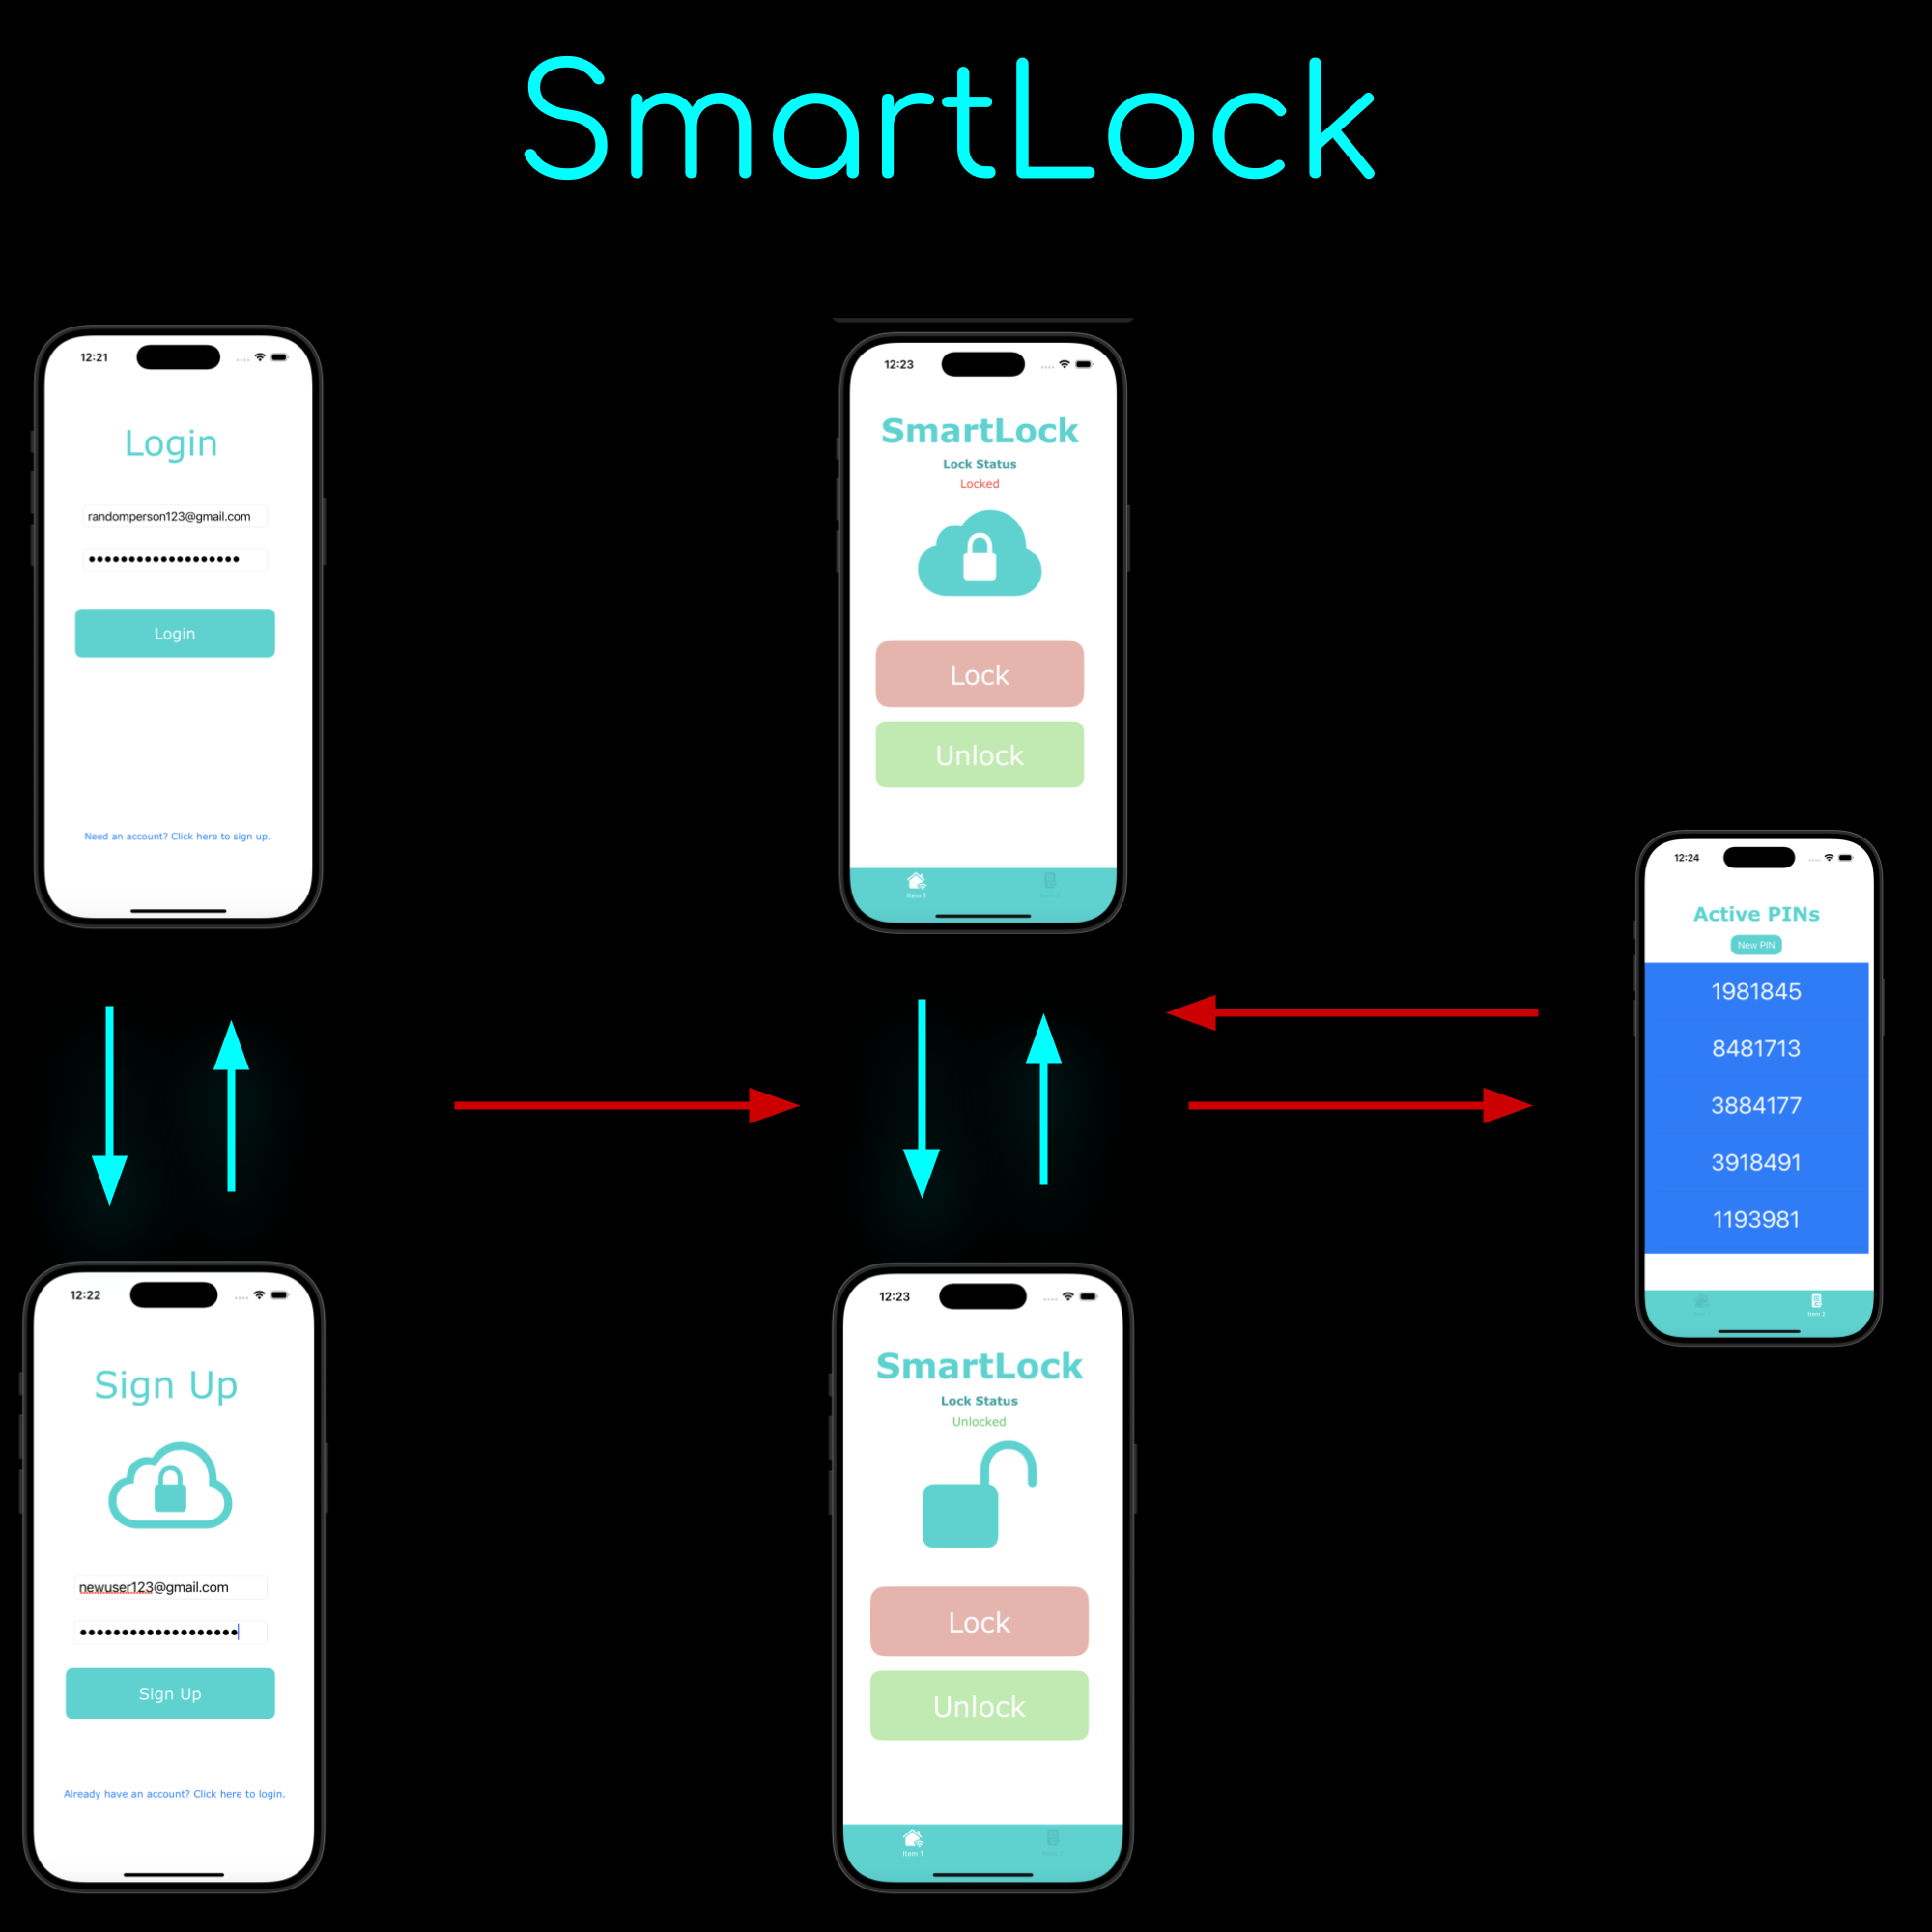
\includegraphics[width=100mm,scale=0.1]{./img/flowsl.png}
\end{center}

\subsection{\textcolor{gray}{Economic Analysis}}
\subsection{\textcolor{gray}{Outstanding Issues}}
\section{Appendices}
\subsection{\textcolor{gray}{Models and Simulations}}
\subsection{\textcolor{gray}{Decision Table Inputs}}
\subsection{\textcolor{gray}{Test Plan}}

\textcolor{teal}{\subsection*{Scope}}
\subsubsection{Firebase Mobile Connectivity Test}
\subparagraph{Test Goals and Purpose}
\begin{itemize}
    \item Ensure that an IOS device can securely connect and push data to the Firebase Firestore servers.
    \item What happens when there may be bad network connection
    \item Set a certain time frame for the pin to be qualified for
\end{itemize}

\subparagraph{Parameters}
\begin{itemize}
    \item 1/0 LOCK$\_$STATE necessary for defining lock-state, 1 is unlocked, 0 is locked.
    \item 7 digit QUALIFIED$\_$PIN list on an allow list for physical keypad on SmartLock.
    \item Make sure what data we send from phone is on firebase
    \item Provide time frame as input for start and expiration time for pin code
\end{itemize}

\subparagraph{Expectations of Test}
\begin{itemize}
    \item There will be no issue with pushing a simple piece of data for LOCK$\_$STATE to the firestore servers, clicking lock will properly push a 0 and clicking unlock will store a 1. Additionally, the pin list composed of generated and custom user pins will also have no trouble being communicated with Firestore servers to later be fetched by the physical device as an additional mechanism for locking and unlocking.
    \item Testing the time frame of the pin code, ensure only the time when valid to use the pin. Otherwise other times should be invalid.
\end{itemize}

\subsubsection{Lock Hardware Functionality Test}
\subparagraph{Test Goals and Purpose}
\begin{itemize}
    \item Ensure that an ESP32-C3 device can securely connect and retrieve data from the Firebase Firestore servers.
    \item Ensure that the ESP32-C3 board can correctly interact with hardware to enable mechanisms for locking/unlocking.
    \item Ensure that invalid codes should not release bolt, while valid codes should.
\end{itemize}


\subparagraph{Parameters}
\begin{itemize}
    \item 1/0 LOCK$\_$STATE necessary for defining lock-state, 0 is locked, 1 is unlocked. Retrieved from firebase.
    \item 7 digit QUALIFIED$\_$PIN list on an allow list for physical keypad on SmartLock.
\end{itemize}

\subparagraph{Expectations of Test}
\begin{itemize}
    \item The locking mechanism will respond appropriately after retrieving from Firestore, and the bolt will trigger when the parameter is set to 0 and likewise release given a 1 value. Additionally, the bolt will release given a valid input from the QUALIFIED$\_$PIN list and reject other non-valid input pins.
    \item Expecting the lock to not unlock after a code is expired, only unlock when it is still valid in a time frame.
\end{itemize}

% Nathaniel's addition

\subsubsection{Multi-User \& Concurrency Test (Low Priority)}
\subparagraph{Test Goals and Purpose}
\begin{itemize}
    \item Ensure that multiple users can simultaneously interact with the smart lock through the mobile app and keypad without causing system conflicts.
    \item Verify that Firebase can handle concurrent updates to the lock state and PIN list without failure.
    \item Ensure the lock responds appropriately when multiple unlock requests are received from different users.
\end{itemize}


\subparagraph{Parameters}
\begin{itemize}
    \item Simultaneous requests from different mobile devices attempting to unlock/lock the door.
    \item Simultaneous PIN entries from different users on the physical keypad and mobile app.
\end{itemize}

\subparagraph{Expectations of Test}
\begin{itemize}
    \item Multiple users attempting to unlock the door at the same time should not cause conflicts or undefined behavior.
    \item The lock should process and execute the most recent valid request, ensuring no delays or duplicate actions.
    \item System logs should correctly track each user’s request, ensuring accountability and reliable data collection for user feedback.
\end{itemize}
% End Nathaniel's addition
\newpage

% New Section ----------------------------------------------------------------------------------------
\textcolor{teal}{\subsection*{Administrative Details}}

\subsubsection{Firebase Mobile Connectivity Test}
\textbf{\textit{Date $\&$ Location:}} Mar 12, 2025 in class
\newline
\textbf{\textit{Conducting Test:}} Jackson Kennedy, Adam Wu, Nathaniel Laurente, Neena Nguyen, and Professor Harrison.

\subsubsection{Lock Hardware Functionality Test}
\textbf{\textit{Date $\&$ Location:}} Mar 31, 2025 in class
\newline
\textbf{\textit{Conducting Test:}} Jackson Kennedy, Adam Wu, Nathaniel Laurente, Neena Nguyen, and Professor Harrison.

\subsubsection{Multi-User \& Concurrency Test}
\textbf{\textit{Date $\&$ Location:}} April 18, 2025 in class
\newline
\textbf{\textit{Conducting Test:}} Jackson Kennedy, Adam Wu, Nathaniel Laurente, Neena Nguyen, and Professor Harrison.

\textcolor{teal}{\subsection*{Design of Experiment}}
\subsubsection{Firebase Mobile Connectivity Test}
\textbf{\textit{Testing method type:}} Functional Testing, does the simple job of sending unlock or lock to firebase server, also sending pins.
\newline
\textbf{\textit{Test apparatus:}} Firebase Cloud service
\newline
\textbf{\textit{Independent Variables:}} Lock Status, Acceptable Pins
\newline
\textbf{\textit{Dependent Variables:}} N/A
\newline
\textbf{\textit{Number of factors:}}
\newline
\textbf{\textit{Sampling Procedures:}} 2 samples of observing Firestore for 1/0 LOCK$\_$STATE. 2 randomly generated PINs and 1 custom-user pin.

\subsubsection{Lock Hardware Functionality Test}
\textbf{\textit{Testing method type:}} When phone sends data for unlock or lock onto firebase, the lock should quickly retrieve information and respond accordingly. The purpose of this is to make sure the lock receives the data fast enough so that people waiting outside the lock does not wait too long for door to unlock. This should also be similar for the pin code case.
\newline
\textbf{\textit{Test apparatus:}} Utilize ESP32-C3 alongside a Solenoid door lock.
\newline
\textbf{\textit{Independent Variables:}} Make sure that the ESP32-C3 can read a simple "Hello world" on the server for basic testing.
\newline
\textbf{\textit{Dependent Variables:}} Everytime we are generating a new code from phone to firebase, the ESP32-C3 should also be able to retrieve those codes as valid codes immediately.
\newline
\textbf{\textit{Number of factors:}} N/A factors considered in this moment
\newline
\textbf{\textit{Sampling Procedures:}} Samples obtained from servers for LOCK\_STATE, only 0 or 1. Then we have samples for pin codes as well from Firebase.
\newline

\subsubsection{Multi-User \& Concurrency Test}
\textbf{\textit{Testing method type:}} Multiple phones will send an unlock signal from phone at nearly the exact same time and see if any undefined behavior occurs. Send a lock signal and an unlock signal at the same time to test if we can prioritize actions that came first, or lock the app after an action from one device has been made.
\newline
\textbf{\textit{Test apparatus:}} Mobile Device along with ESP32-C3.
\newline
\textbf{\textit{Independent Variables:}} Make sure that the ESP32-C3 can read a simple "Hello world" on the server for basic testing.
\newline
\textbf{\textit{Dependent Variables:}} ESP32-C3 behavior after multiple devices send a signal at the same time or immediately one after the other.
\newline
\textbf{\textit{Number of factors:}} 2 factors to be considered
\newline
\textbf{\textit{Sampling Procedures:}} Samples obtained from servers for LOCK\_STATE, only 0 or 1. Determine if multiple signals causes undefined or expected behavior.



\textcolor{teal}{\subsection*{Testing Procedures}}
\subsubsection{Safety Precautions}
Safety precautions for our project includes not having fast and forceful locks that can hurt individuals.

\subsubsection{Data Collection Method}
Collect data from the phone providing the custom pins onto firebase, as well as collecting data for locking or unlocking. We will also note down which users are grouped together to be able to use the same pin for unlcocking door.

\subsubsection{Observation of External Factors}
Some external factors that could make our product not function properly could include:

\begin{itemize}
    \item Bad network connection from phone or from ESP32-C3
    \item Firebase not loading properly
\end{itemize}
\subsection{\textcolor{gray}{Results}}
\textcolor{teal}{\subsection*{Summary Tables}}
\renewcommand{\arraystretch}{1.3} % Adjust row height


\begin{table}[h]
    \centering
    \rowcolors{2}{teal!10}{teal!25}
    \begin{tabular}{|l|c|c|p{4.5cm}|}
        \hline
        \rowcolor{teal!50}
        \textbf{Objective ( Target )} & \textbf{Result} & \textbf{Met?} & \textbf{Discussion} \\
        \hline
        Firebase Connectivity & Appropriate 1/0 & N/A & Half this test done - explain how lock/unlock work but havent tested PINs yet \\
        
        Lock Hardware Functionality & N/A -\textit{Mar 31, 2025} & N/A & While this test has not been conducted yet, we suspect we will pass this test as the Firebase - Firestore lock/unlock was already successful, and the appropriate data was well-received by the ESP32-C3. All that remains is to ensure that the solenoid lock responds properly to an input signal, as well as compares and responds accordingly to valid/invalid codes. \\
        
        Concurrency & N/A -\textit{April 18, 2025} & N/A & While this test has not been conducted yet, we suspect that we will pass this test. Firebase should be able to handle multiple calls close to each other, as well as transmit this signal in the appropriate order. The Firestore database updated extremely quickly in real-time and shouldn't have trouble with concurrent calls. The PIN entries from different users also shouldn't cause conflict, and the door should unlock/lock as intended. \\
        
        \hline
    \end{tabular}
\end{table}

\end{document}